The algorithm for obstacle avoidance needs to avoid cylindrical objects in a 3D space. Specifically, it needs to be able to avoid obstacles by going around them - this is more efficient when doing the automatic flight portion. However, for the ODLC survey, the aircraft should fly over the obstacles to keep the survey path intact. The algorithm needs to take into account the size of the aircraft plus an additional safety factor during the avoidance in case of GPS accuracy when considering possible collisions and acceptable routes .

All the algorithms are housed in the ‘avoidance’ module within the GCOMv2 software in the GCS. It contains a variety of REST endpoints to perform routing on the map frontend. Some preprocessing is done as soon as the information is gathered from interop, however the actual routing is done on demand to keep system resource use efficient. Once routing is complete, the waypoints are cached to the database so that future calls don’t need to perform the routing again. There is an endpoint to force a re-compute of the route, as well as too write a custom path to the database cache. This allows for user modifications if the computer generated route is unsatisfactory.

The core algorithm for the avoidance and routing is based of a modified version of the A* algorithm called L1. The A* algorithm treats the flight space as a 2D grid, and is computed as a graph. The A* algorithm starts at the start node of the graph then recursively tries all possible routes through the edges of the grid, however it prioritizes trying the path that is both the shortest path so far and what it thinks is the best possible next path. This best next path is controlled by a heuristic. In this case it is the straight line distance from the node to the goal. The advantage of using this path finding algorithm to do obstacle avoidance is that any combination or layout of obstacles can be handled without the inclusion of special rules or edge cases. It also works easily in three dimensions, so it can handle the full flight space and all of the problem requirements.

\begin{figure}[h]\centering
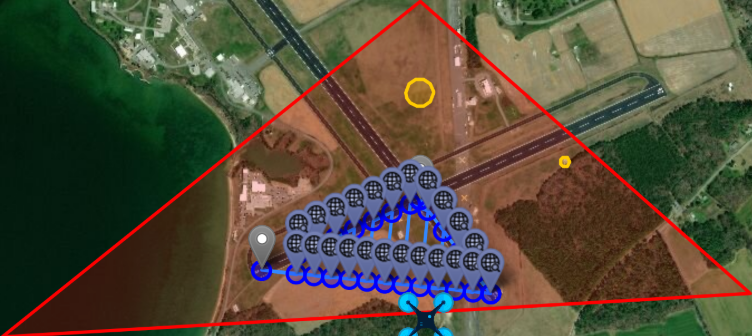
\includegraphics[width=\linewidth]{figures/OA_1.png}
\caption{The target route. Flyzone in red, obstacles in yellow.}
\label{fig:OA_1}
\end{figure}

However, for UAS's use case the base A* algorithm was improved. Inspiration was taken from the L1 improvement of the A* algorithm. Mainly, the steps of pre-processing the grid and reducing the number of potential paths that need to be considered. In the case of this problem, the points of the 1m by 1m grid were reduced to just the nodes of: the waypoints given, a few points close to the obstacles and points around the inside edge of the flyzone (Figure 2). This greatly reduces the number of points and paths considered and considerably speeds up the routing. To further speed up the routing, the edges of the graphs between the points were pre-computed to reduce the pathfinding time even more. This is done asynchronously immediately after the mission information is gathered from the interop server.

\begin{figure}[h]\centering
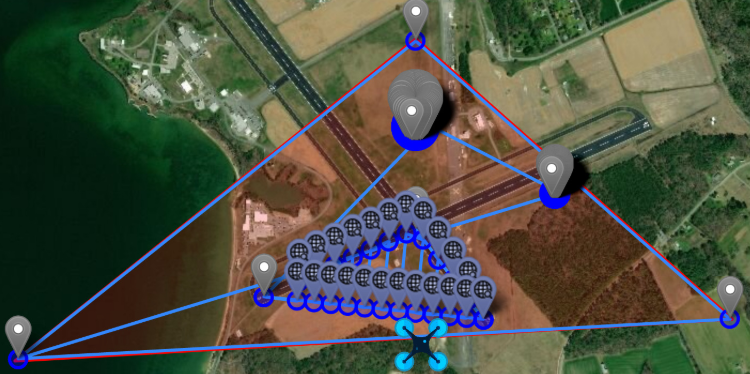
\includegraphics[width=\linewidth]{figures/OA_2.png}
\caption{The reduced graph of nodes used in the A* search.}
\label{fig:OA_2}
\end{figure}

In Figure \ref{fig:OA_2}, note the clusters of overlapping nodes around the obstacles. To enable 3D searching, but still reduce the number of nodes tested, the search nodes are placed just outside the mid height of the obstacle, and just above the top of the obstacle. On the map they appear as overlapping nodes.

When testing the algorithm, several key edge cases between two points were considered:
\begin{itemize}
\item Free Path between two points.
\item Single obstacle.
\item Multiple obstacles in a line.
\item Multiple obstacles coincident.
\item Multiple obstacles overlapping.
\item Multiple obstacles randomly dispersed.
\item Going around and going over obstacles.
\item Flyzone jutting out between the two points.
\item Combinations of the above.
\end{itemize}

\endinput


